
%(BEGIN_QUESTION)
% Copyright 2011, Tony R. Kuphaldt, released under the Creative Commons Attribution License (v 1.0)
% This means you may do almost anything with this work of mine, so long as you give me proper credit

A heat exchanger is used to lower the temperature of sulfuric acid (H$_{2}$SO$_{4}$) exiting an exothermic reactor in an acid manufacturing process, using water as the coolant.  An automatic control valve will eventually be installed in the water line, but for now a hand (manual) valve performs the role of coolant throttling over a range of 0 to 25 GPM (gallons per minute):

$$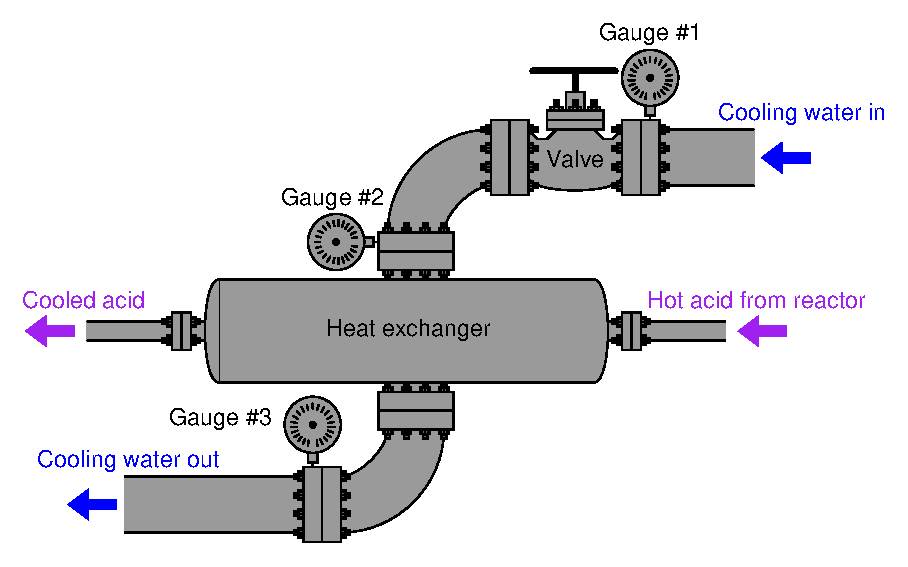
\includegraphics[width=15.5cm]{i03410x01.eps}$$

An experienced instrument technician is summoned to test this heat exchanger system and determine what kind of valve characterization (quick-opening, linear, equal-percent) is best for throttling the water flow.  The technician proceeds to set the manual valve to different positions while recording the three pressure gauge readings and the flow rate (measured by a flowmeter not shown in this illustration).  The results are shown in this table:

% No blank lines allowed between lines of an \halign structure!
% I use comments (%) instead, so that TeX doesn't choke.

$$\vbox{\offinterlineskip
\halign{\strut
\vrule \quad\hfil # \ \hfil & 
\vrule \quad\hfil # \ \hfil & 
\vrule \quad\hfil # \ \hfil & 
\vrule \quad\hfil # \ \hfil \vrule \cr
\noalign{\hrule}
%
% First row
Water flow & Gauge \#1 & Gauge \#2 & Gauge \#3 \cr
%
\noalign{\hrule}
%
% Another row
0 GPM & 83 PSI & 0 PSI & 0 PSI \cr
%
\noalign{\hrule}
%
% Another row
15 GPM & 83 PSI & 1.1 PSI & 0.4 PSI \cr
%
\noalign{\hrule}
%
% Another row
25 GPM & 82 PSI & 2.0 PSI & 0.6 PSI \cr
%
\noalign{\hrule}
} % End of \halign 
}$$ % End of \vbox

Interpret these pressure measurements to select the best control valve characterization for the task ({\it linear}, {\it equal percentage}, or {\it quick-opening}), explaining your rationale.

\vfil 

\underbar{file i03410}
\eject
%(END_QUESTION)





%(BEGIN_ANSWER)

This is a graded question -- no answers or hints given!

%(END_ANSWER)





%(BEGIN_NOTES)

A general principle to keep in mind is that a linear-trim valve will respond linearly (flow proportional to stem position) only if the pressure drop across that valve is constant or nearly constant throughout the stem's travel range.  If this is not the case, a different characteristic should be chosen for the valve to ``linearize'' its behavior.

\vskip 10pt

A {\it linear} characteristic is best for this application, because here the valve's $\Delta P$ hardly changes throughout the control range.  This nearly-constant pressure drop will allow a linear control valve to provide a nearly linear flow response.

If, on the other hand, we saw that the pressure difference across the valve varied substantially from 0 GPM to 25 GPM, we might want to choose an equal-percentage control valve characteristic instead of linear.

%INDEX% Final Control Elements, valve: characterization

%(END_NOTES)


